\documentclass{article}
\usepackage{graphicx}
\usepackage{hyperref}
\usepackage[margin=0.75in]{geometry}
\usepackage[utf8]{inputenc}
\usepackage{indentfirst}


\setlength{\parindent}{4em}
\setlength{\parskip}{1em}
\renewcommand{\baselinestretch}{2.0}

\begin{document}
\title{BIOS 611 Project 1}
\author{Jane She \\ e-mail: jane.she@unc.edu}
\date{19 October 2021}
\maketitle

\section{Introduction}


Men's college basketball is a widely popular sport, especially at the Division 1 level and is broadcasted nationally for fans to watch. According to Cav's Corner, the UVA men's basketball team is one of the top revenue generators for the school. 

As a recent graduate of the University of Virginia, I was interested in looking at various game statistics and their infuences on the number of games won by a team. I specificially looked at the 2019 NCAA D1 basketball season since that is both the year that UVA won the national championships and the last pre-COVID season.

In this report, I examined the relationship between the number of games won and statistics including adjusted offensive efficiency, adjusted defensive efficiency, effective field goal percentage, turnover rate, and steal rate.

\section{Data}

The dataset with variable descriptions and more context can be found \href{https://www.kaggle.com/andrewsundberg/college-basketball-dataset}{here} and was found on kaggle. Originally, the data was scraped from barttorvik.com, a famous college basketball website. 

\section{Exploratory Data Analysis}

In our exploratory data analysis, I decided to choose a couple variables I was interested in and plot them against the number of wins. The variables I included are adjusted offensive efficiency, adjusted defensive efficiency, effective field goal percentage shot, turnover rate, and steal rate.

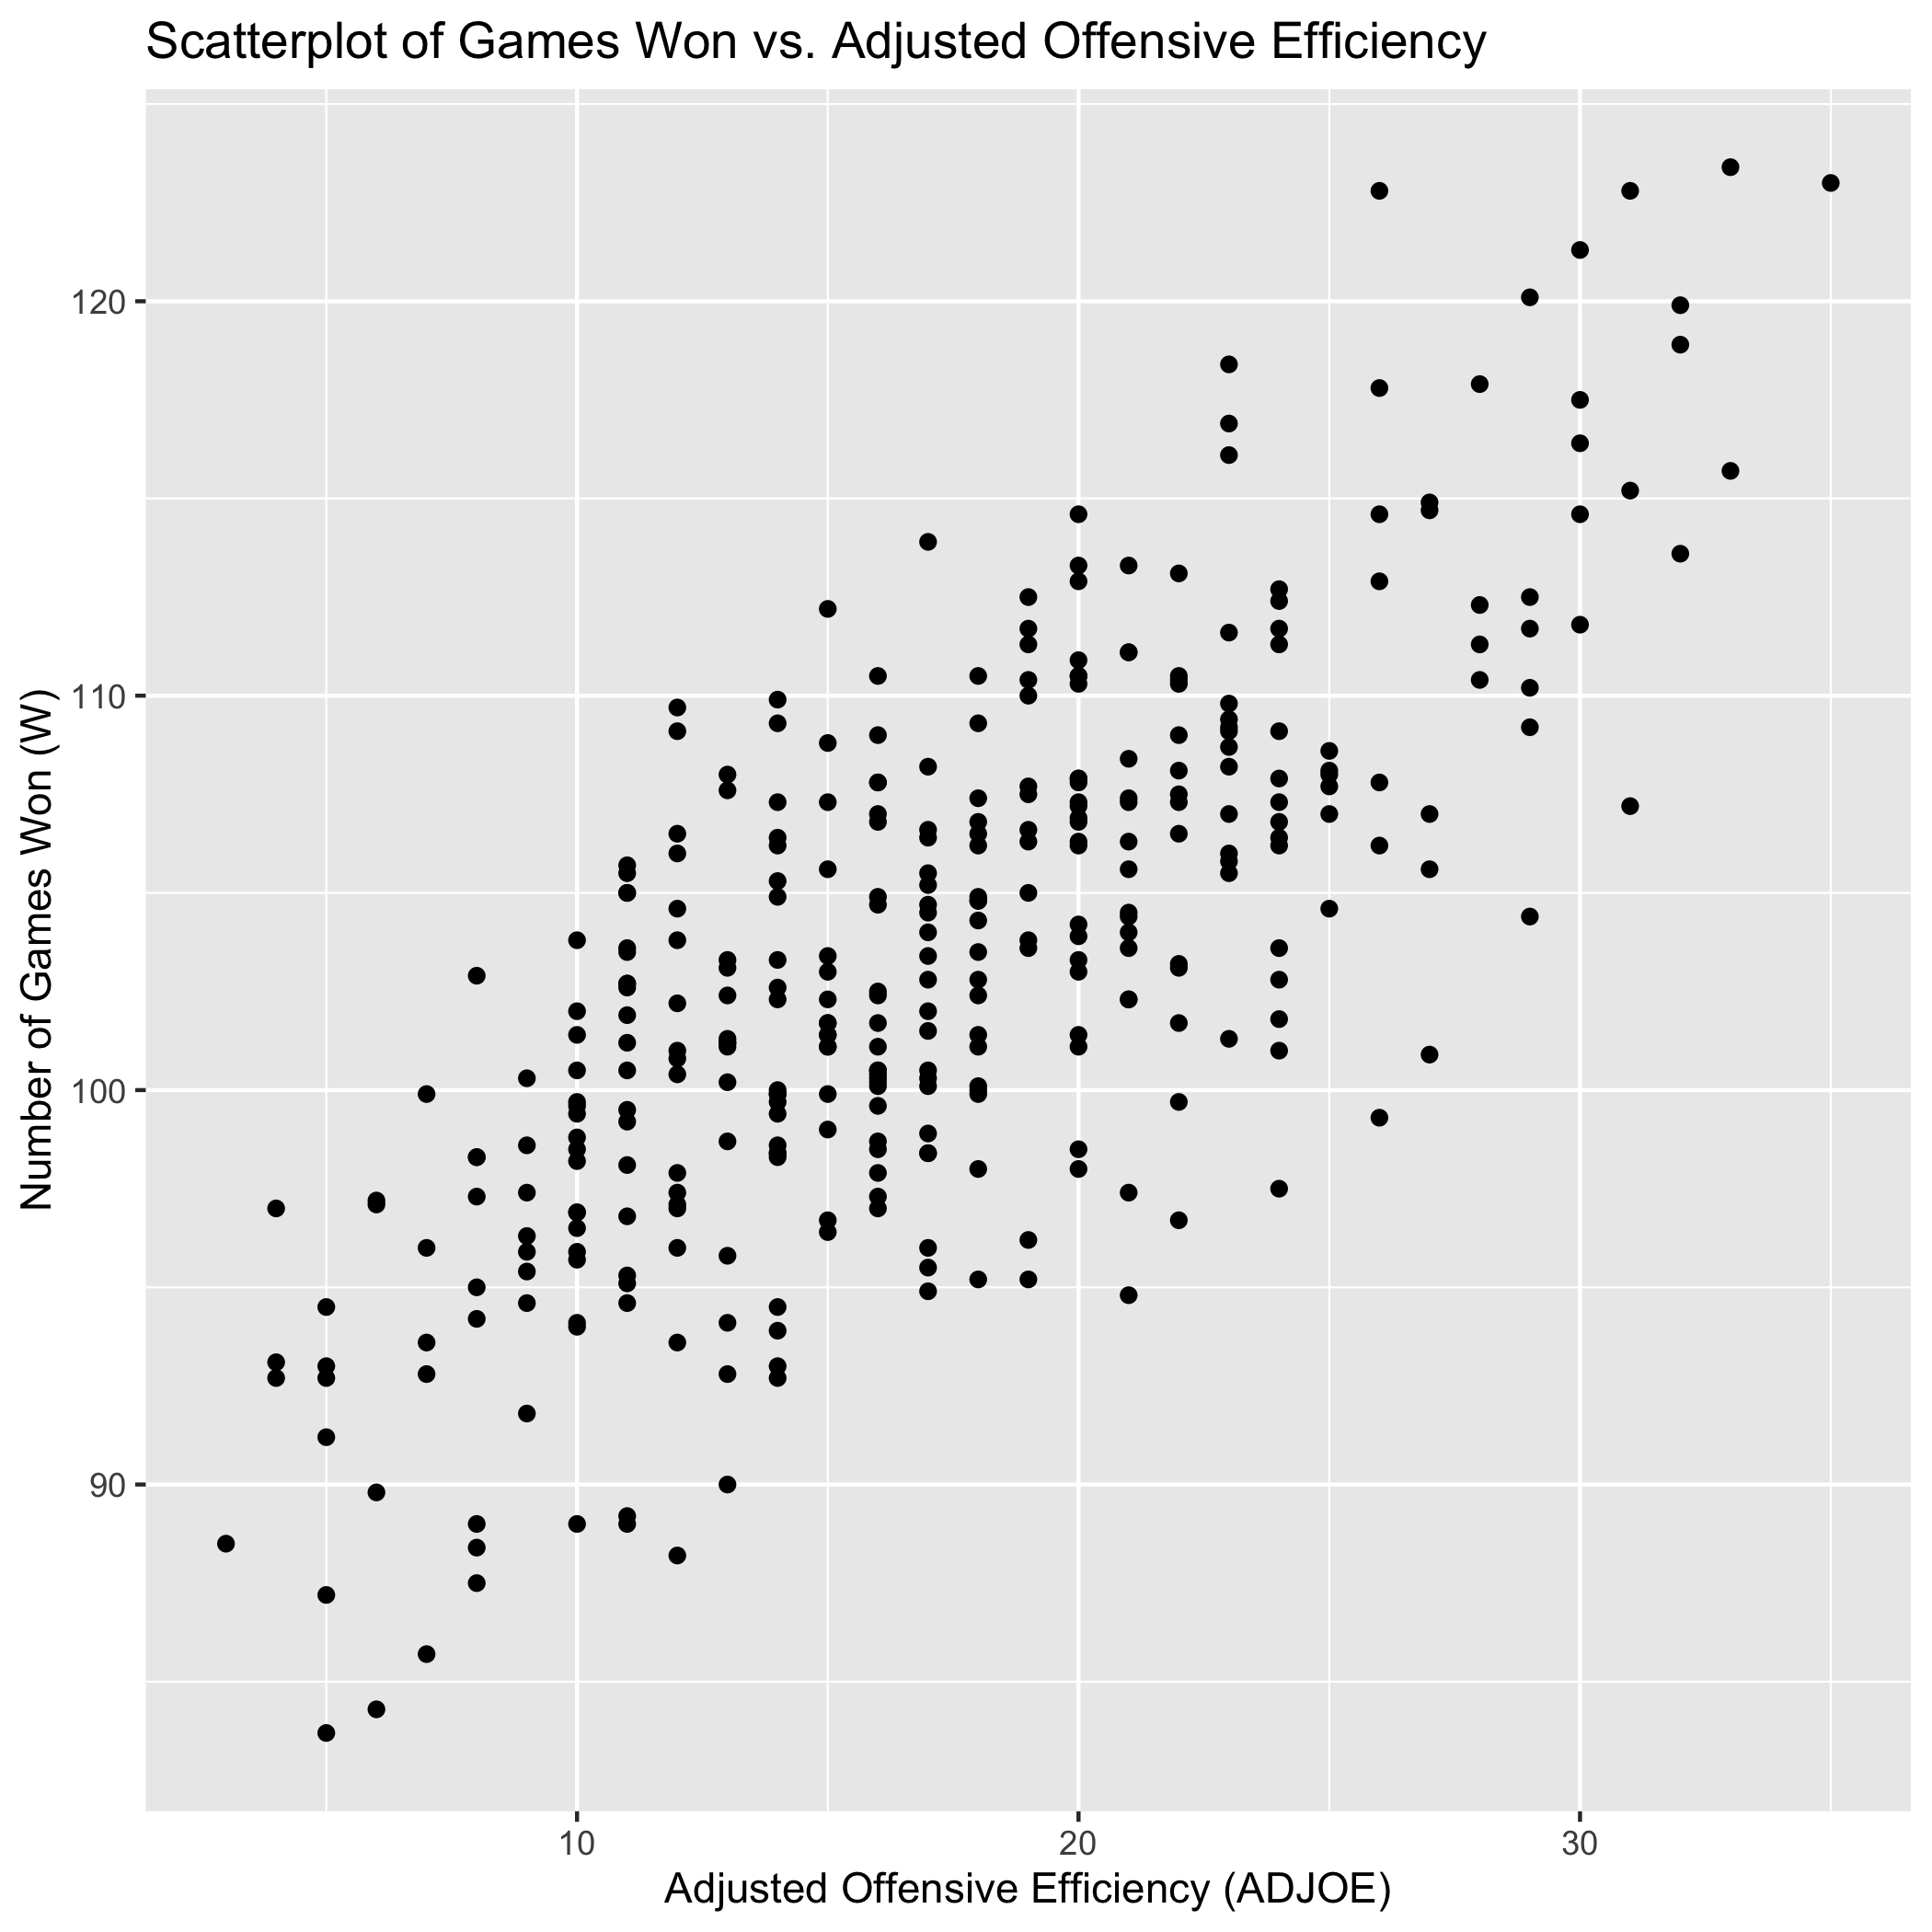
\includegraphics[width=0.5\textwidth]{Figures/W_ADJOE.png}\\
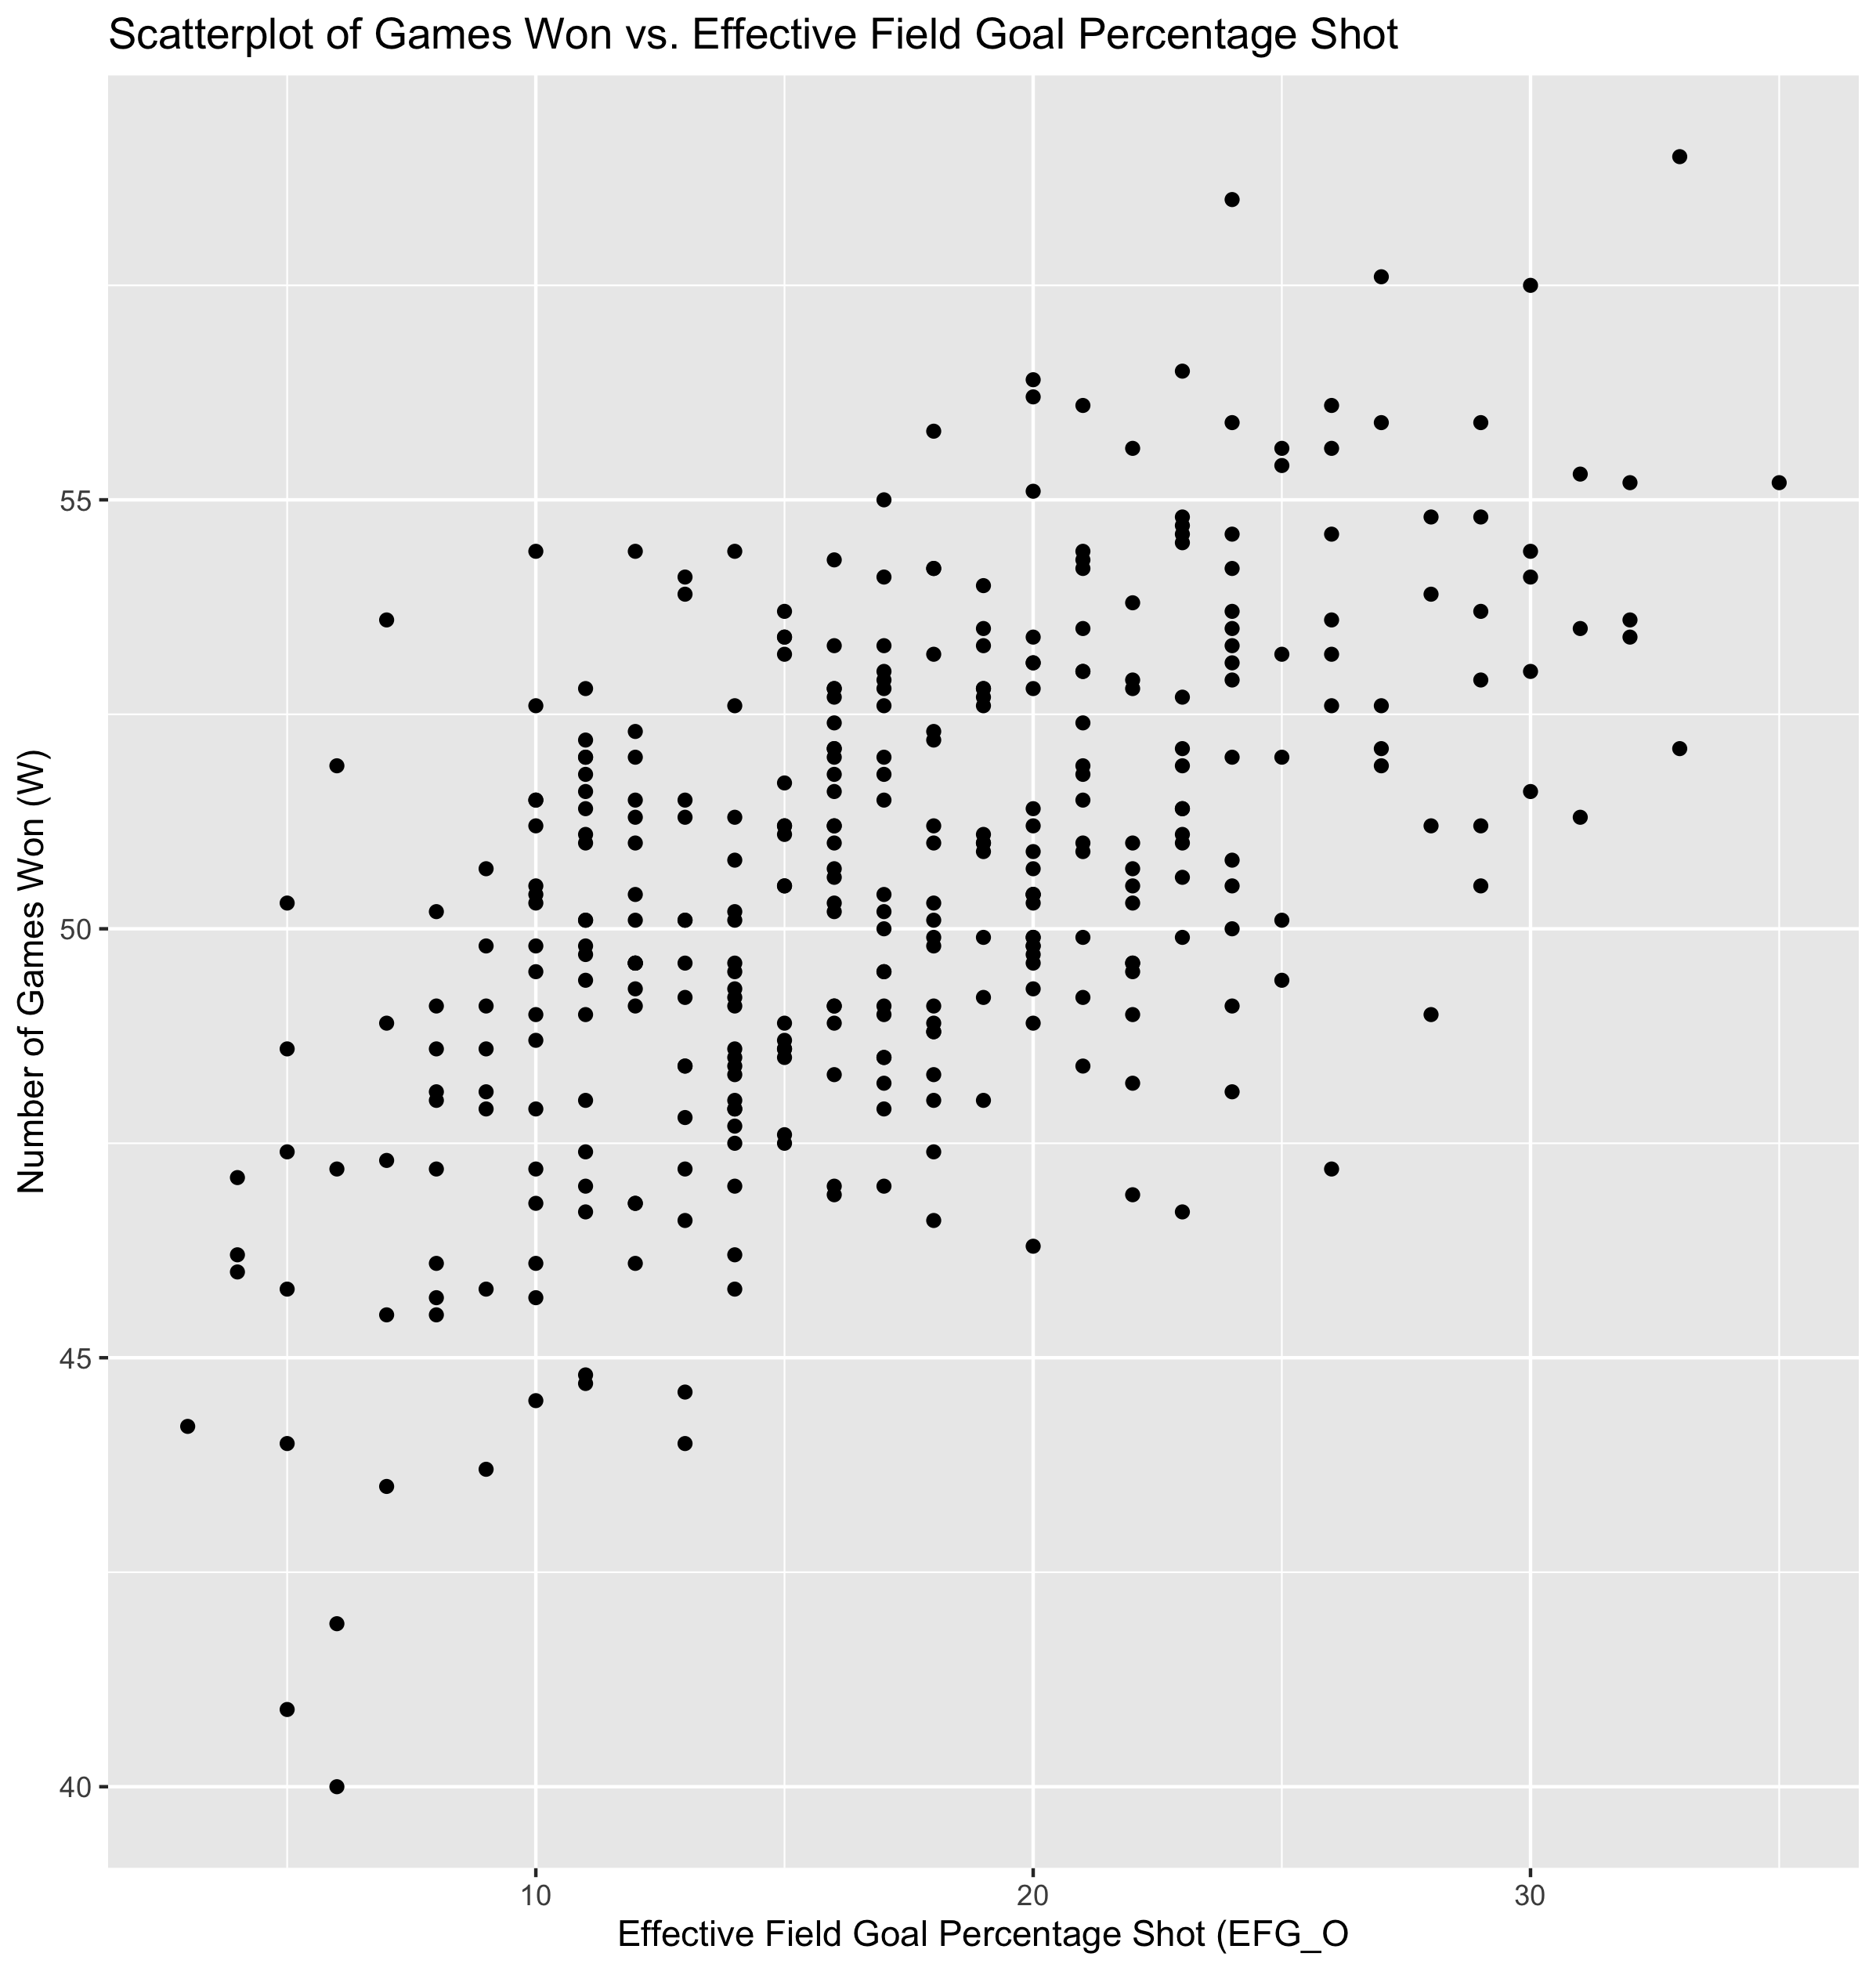
\includegraphics[width=0.5\textwidth]{Figures/W_EFGO.png}\\
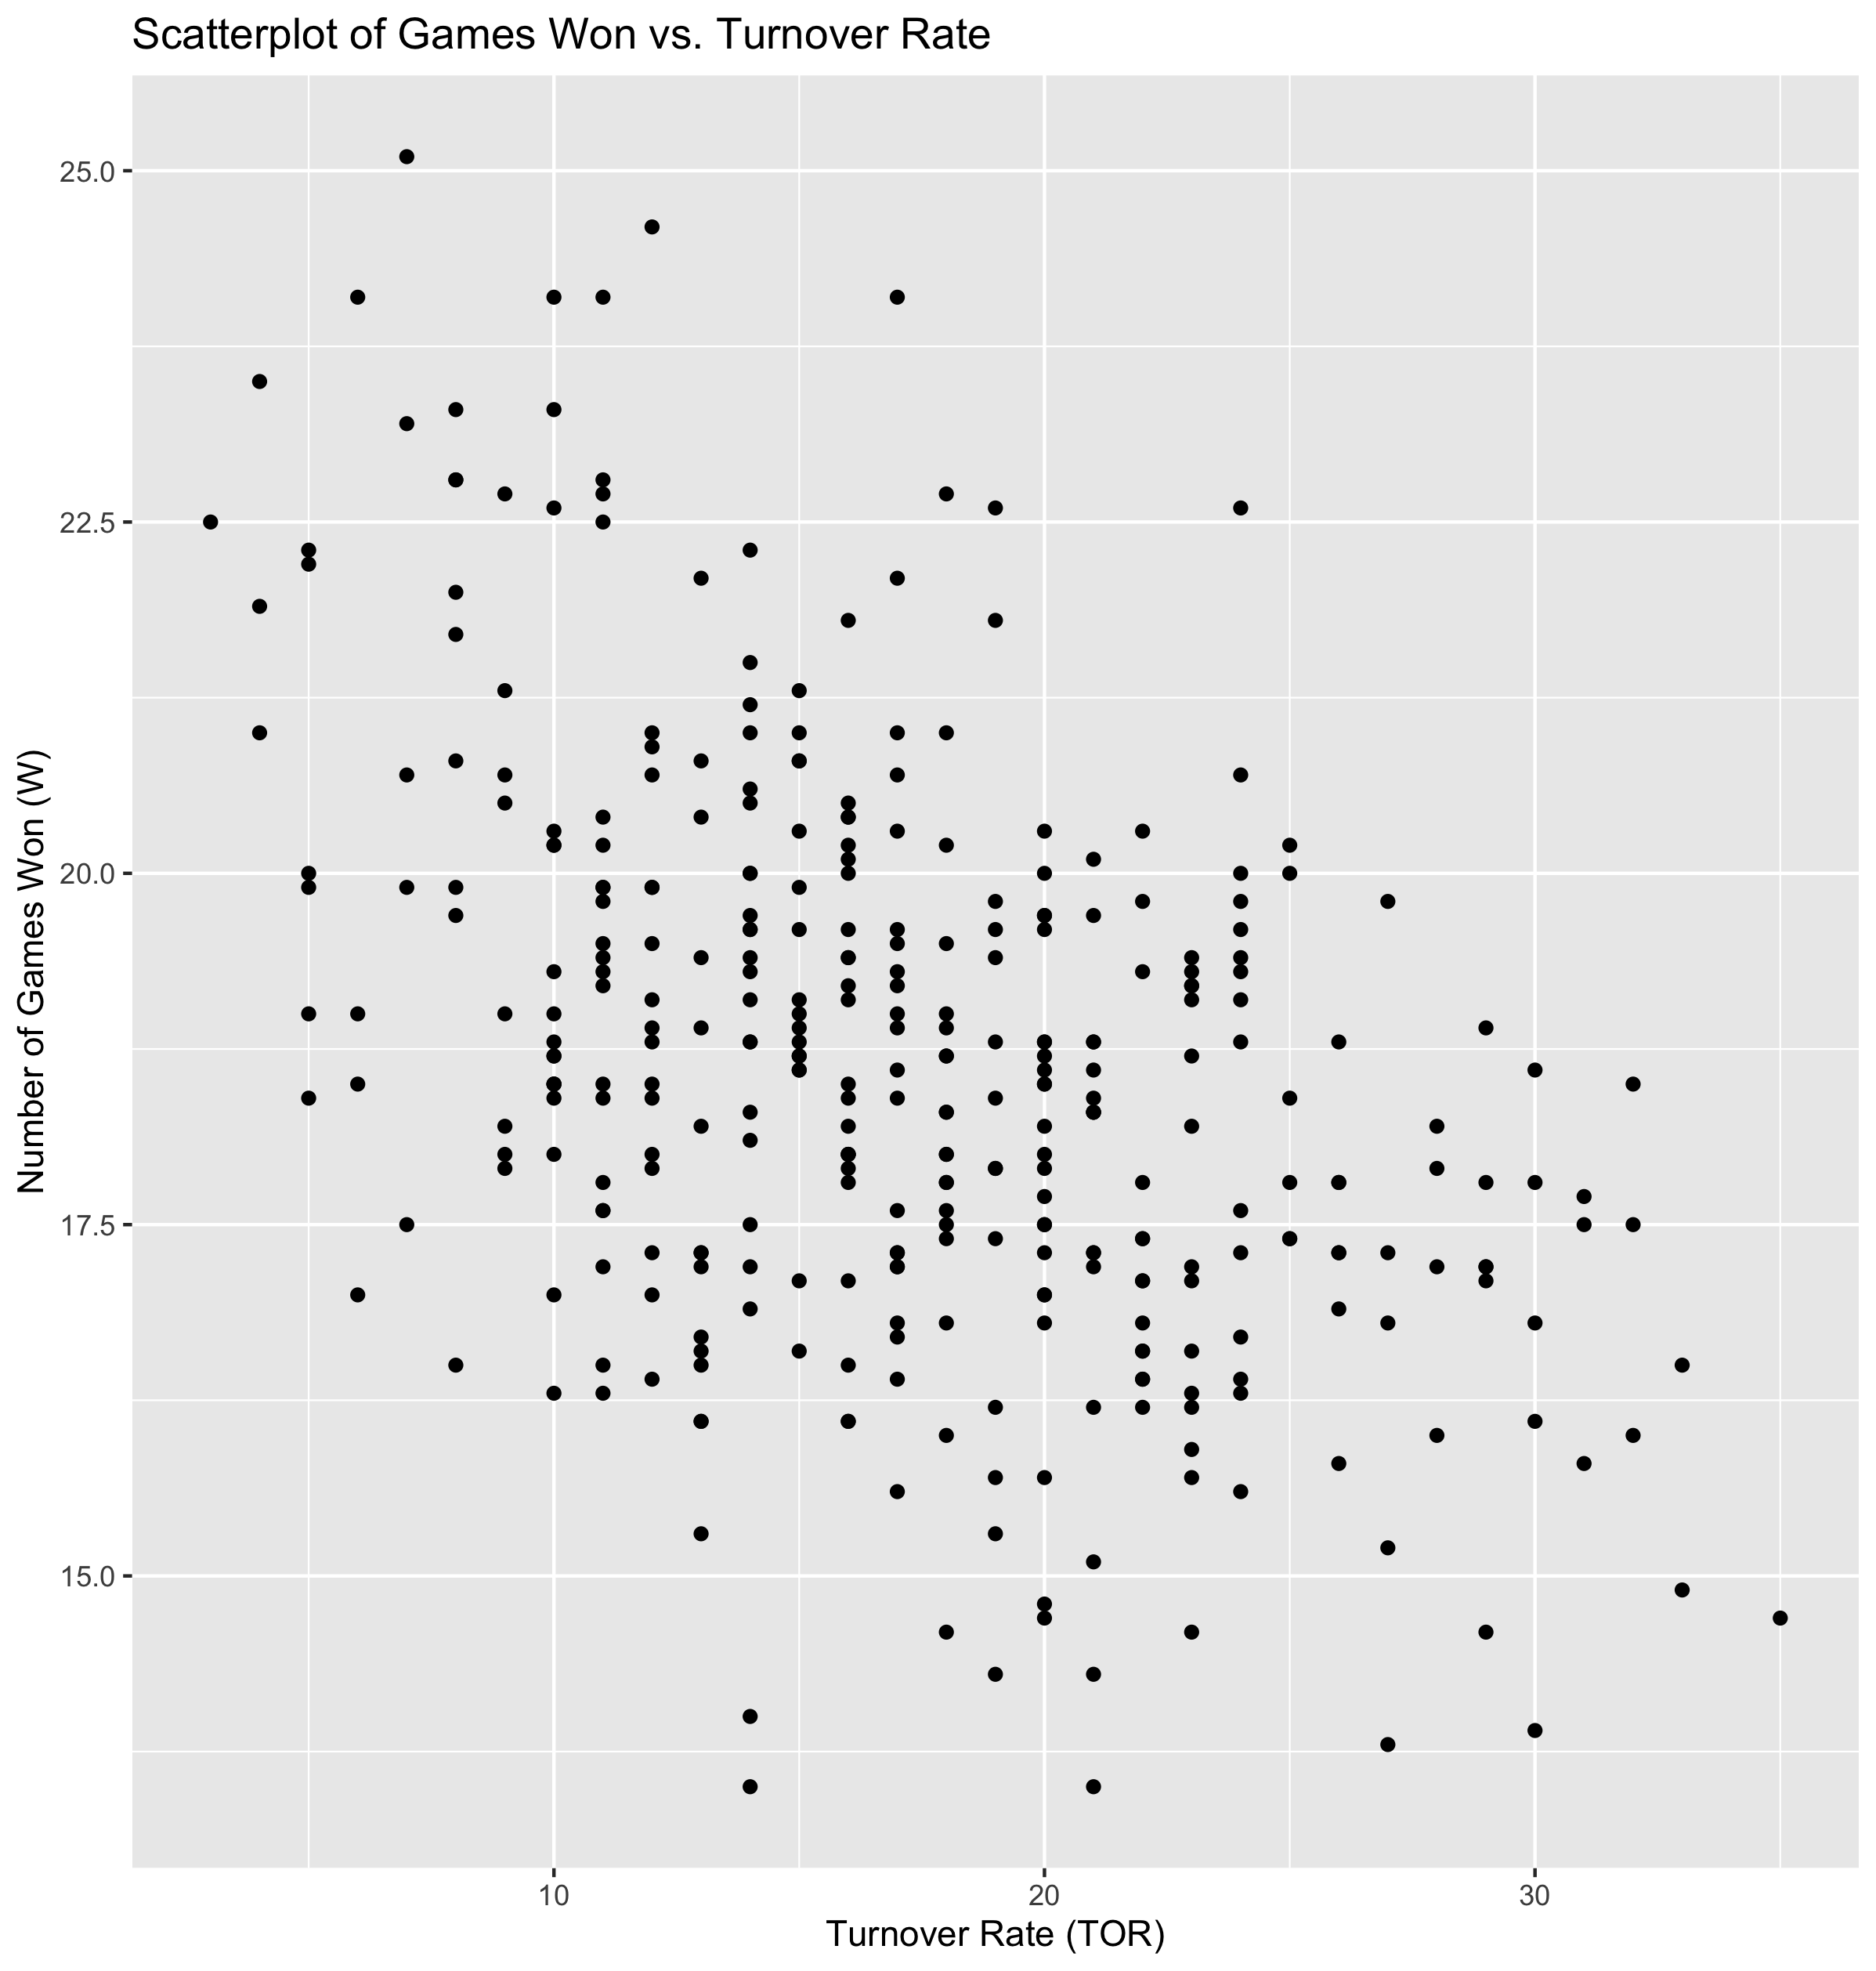
\includegraphics[width=0.5\textwidth]{Figures/W_TOR.png}\\
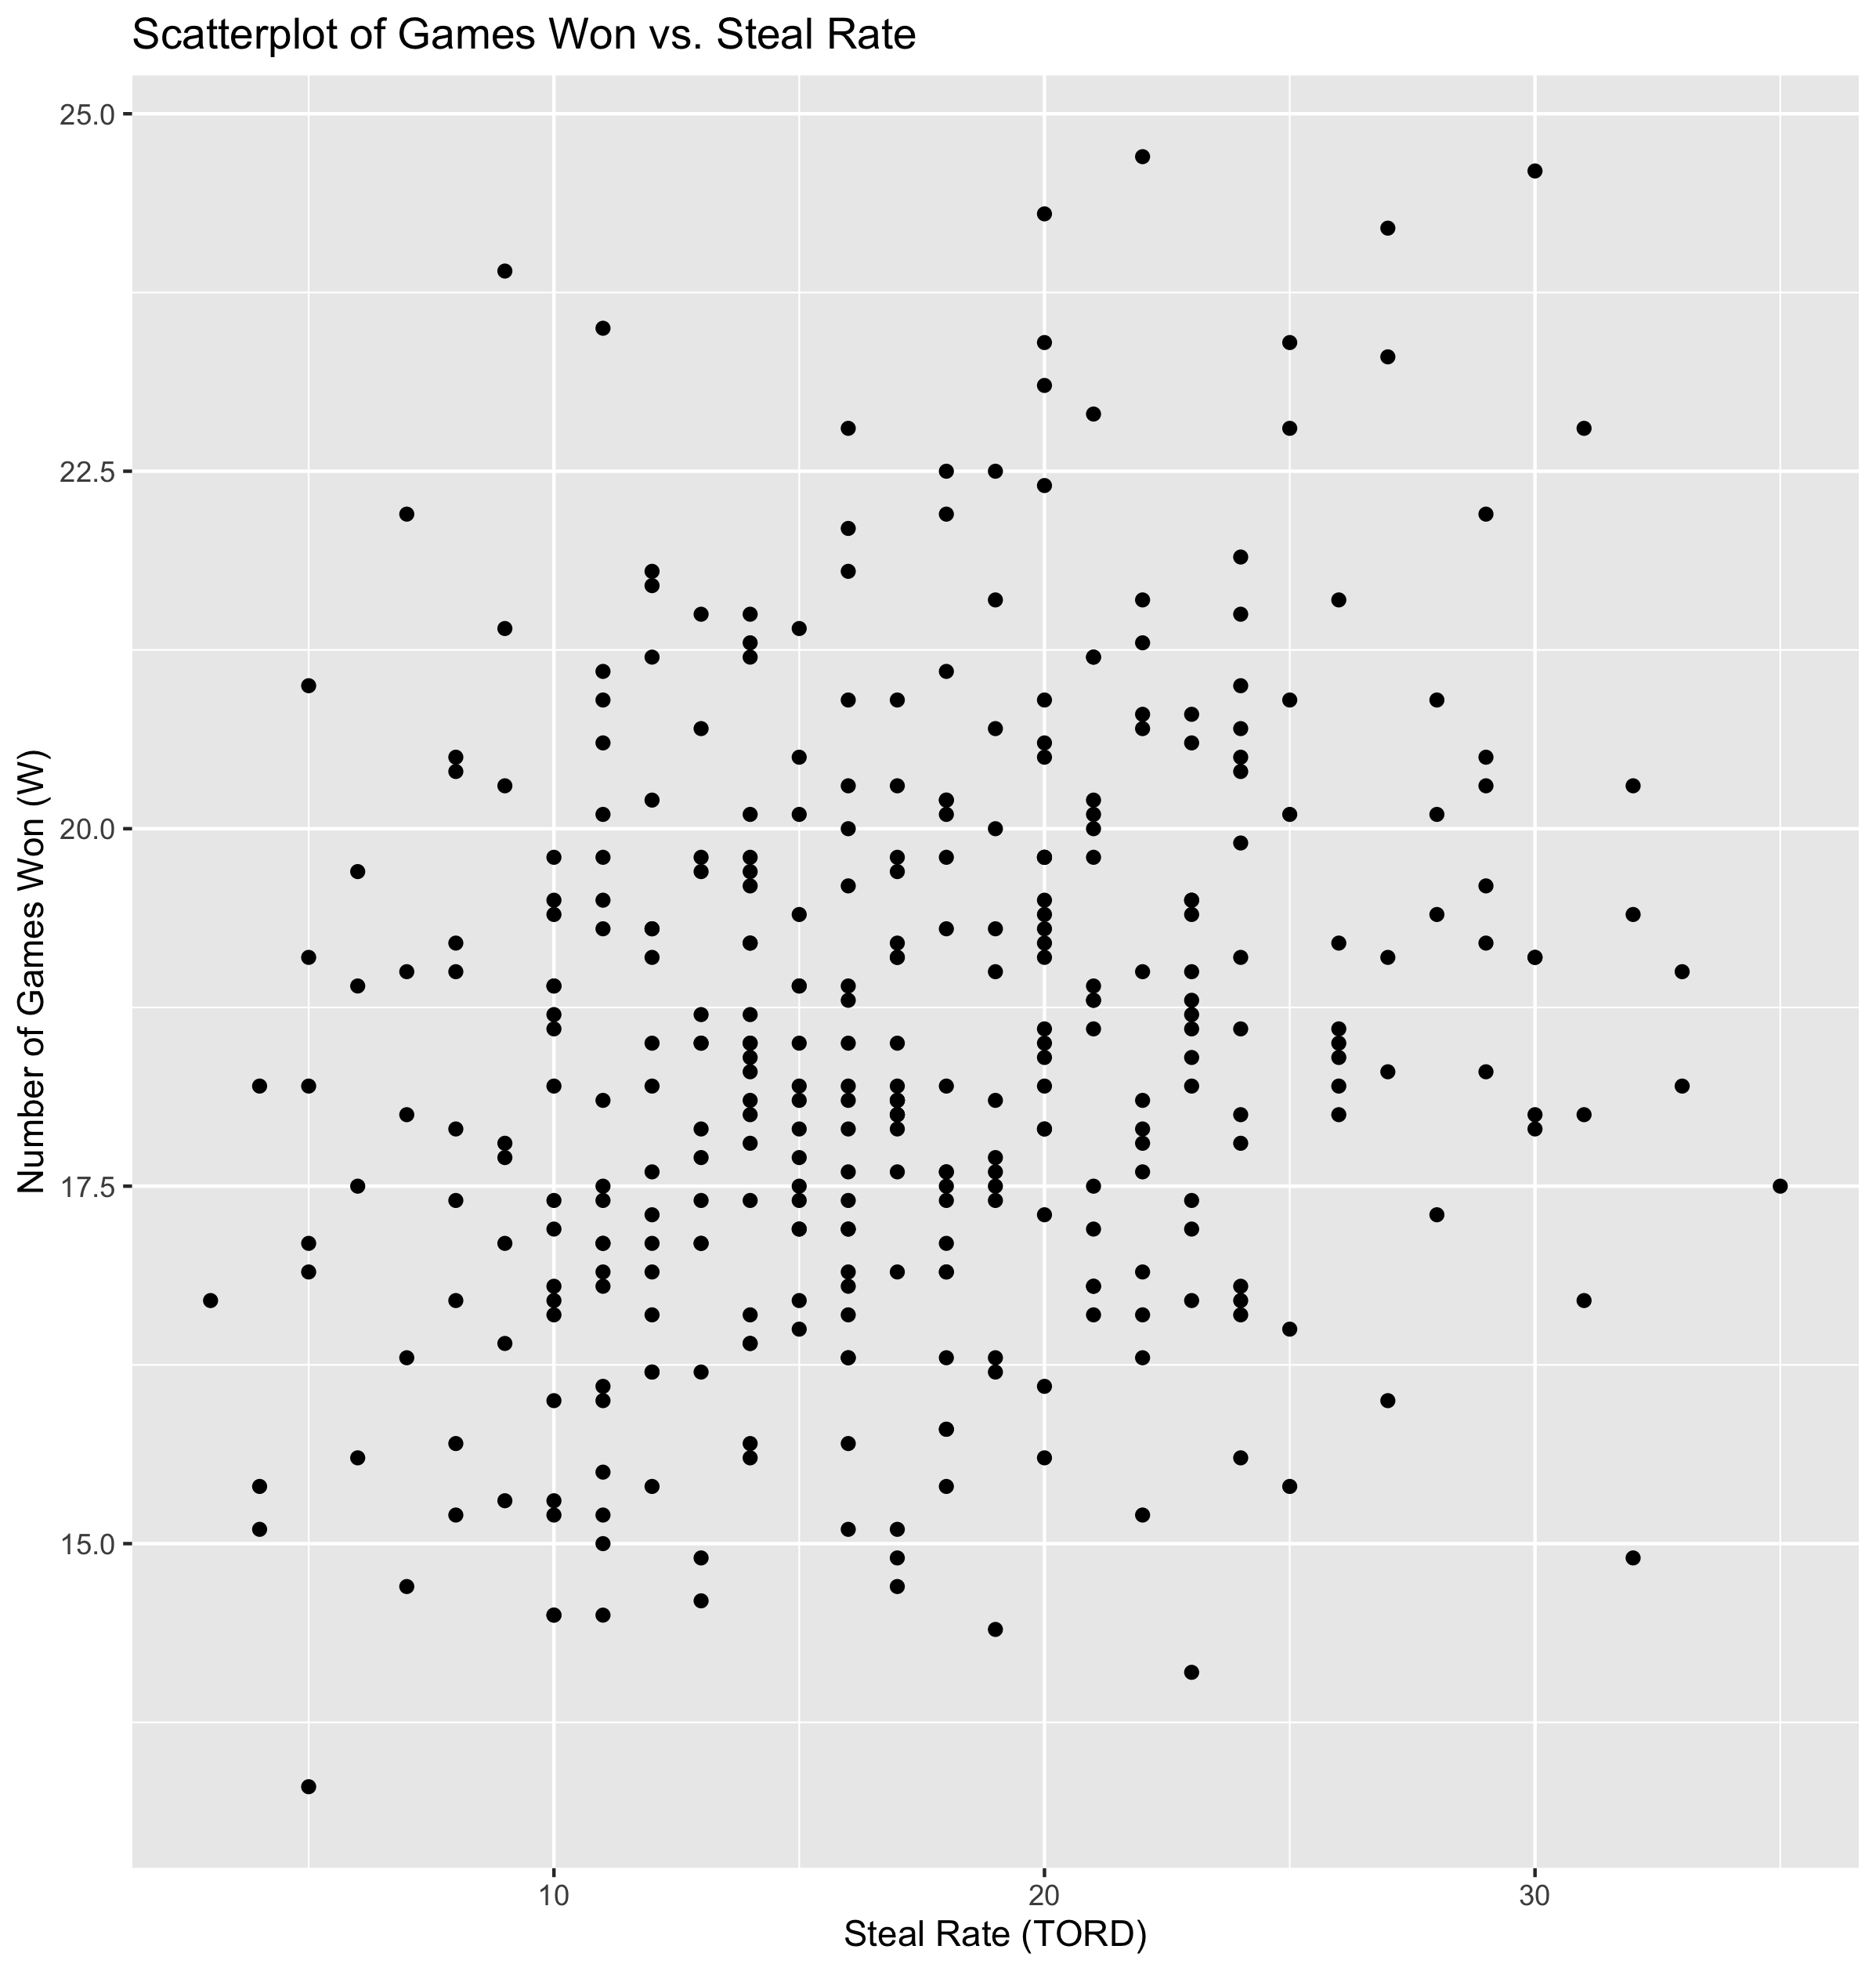
\includegraphics[width=0.5\textwidth]{Figures/W_TORD.png}\\

Additionally, I created a correlation matrix along with a graph of some pairwise interactions.

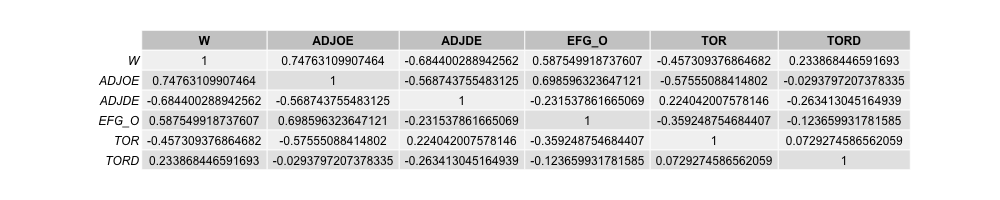
\includegraphics[width=0.8\textwidth]{Figures/correlation_matrix.png}\\

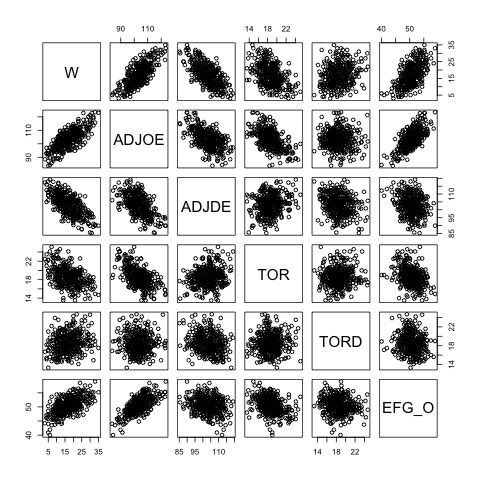
\includegraphics[width=0.8\textwidth]{Figures/pairwise_interaction.png}\\




\end{document}
